\section{E1: Traffic without any obstacle}
The first experiment focuses on the comparison of the GM-PHD filter with the constant detection probability and the GM-PHD
filter
with the dynamic detection probability with different settings explained in Section \ref{sec:mphd_problemDef}. To
analyze
if our proposed method works in common scenarios, videos do not include any obstacle, thus the targets are
constantly visible.

\subsection{V1}
The video \textit{V1} is recorded at 29 fps. For simplicity, only the detections of the right side of the traffic are
taken into the account. This experiment shows frames 36-79 of the video \textit{V1}, as they
includes some interesting situations.
\subsection{V1 -- GM-PHD with the constant detection probability}
The measurements for the GM-PHD filter with the constant detection probability are obtained by the YOLO object detection
model. The parameters' values are displayed in Table \ref{tab:E1-V1-S0}.
\begin{table}[!h]
    \centering
    \begin{tabular}{|c|c|c|c|c|c|}
        \hline
        $P_{D}$ & $P$ & $\sigma_{\upsilon}$ & $\sigma_{\epsilon}$ & $T_p$ & $T_{YOLO}$ \\ \noalign{\hrule height 1.5pt}
        0.9 & $diag(600,600,600,600)$ & 0.1 & 150 & 0.1 & 0.3\\
        \hline
    \end{tabular}
    \caption{The parameter settings for Experiment E1-V1 with the constant detection probability.}
    \label{tab:E1-V1-S0}
\end{table}

Figure \ref{fig:E1-V1-S0} shows some highlights of the GM-PHD filter with the constant detection probability.
\begin{itemize}
    \item \textbf{\ref{fig:E1-V1-S0:01}:} This frame marks the initial state, where four cars have been previously
    identified, thus constituting our observed targets. In the distance, YOLO detects another car; which, however,
    has not yet crossed any spawning point, so it is not included in the observed targets set.
    \item \textbf{\ref{fig:E1-V1-S0:02}:} A new car approaches the scene and is expected to be initialized soon. The
    YOLO model, although overall reliable, occasionally misses certain objects, as demonstrated here with the
    car on the left. With a detection probability of 0.9, this target is pruned from the set and considered lost.
    \item \textbf{\ref{fig:E1-V1-S0:03}:} The previously lost car is, once again, detected. However, it no longer
    falls within the set of observed targets.
    \item \textbf{\ref{fig:E1-V1-S0:04}:} Even though the newly arrived car has crossed the spawning point, the YOLO model
    consistently
    fails to detect it over several frames, resulting in its complete absence from tracking.
    \item \textbf{\ref{fig:E1-V1-S0:05}:} The two cars on the right evade the detection. On this occasion, one
    of the targets manages to persist, allowing for continued tracking of at least one car.
    \item \textbf{\ref{fig:E1-V1-S0:06}:} The previously undetected cars reappear in the frame. Both cars are
    successfully tracked once again.
    \item \textbf{\ref{fig:E1-V1-S0:07}:} Another car enters the scene and is promptly detected and initialized.
    \item \textbf{\ref{fig:E1-V1-S0:08}:} Despite YOLO detecting all the six cars, only three targets are visible in the
    scene. One of the targets encompasses two cars simultaneously, indicating that the GM-PHD filter effectively covers four out of the six targets.
\end{itemize}

In Graph \ref{gr:E1-V1-S0} it is clearly seen that even though the number of targets is increasing, the misdetection
of the YOLO model causes the targets' loss. The "All targets in set" line is fully covered by the blue line, thus the
targets are permanently lost and can not be reborn by a measurement.

This experiment shows that the GM-PHD filter is able to accurately track the position of objects. With the detection
probability $p_D = 0.9$ and without the modified pruning technique, the filter is very sensitive to the capability of
the
object detector and if YOLO is not able to detect all the desired objects, targets can be easily lost.

\begin{figure}[H]
    \centering
    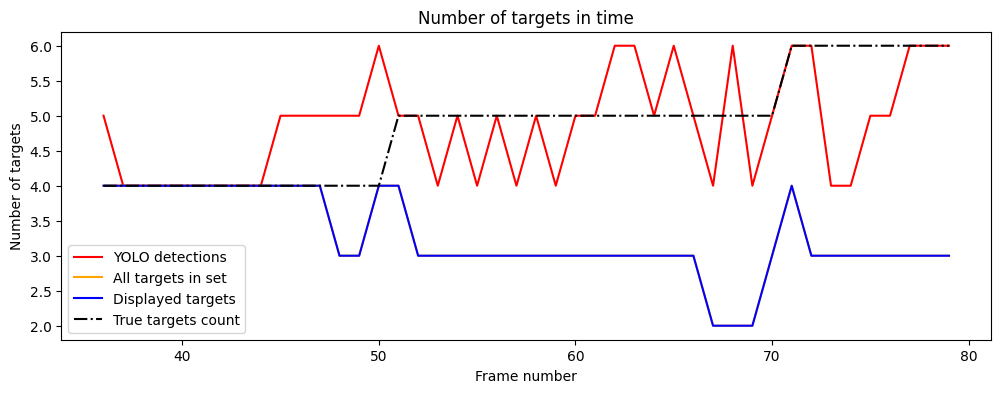
\includegraphics[width=\linewidth]{../../../experiments/E1/V1/noPd/staticPd_det}
    \caption{Development chart of number of detected targets, targets in the filter's queue, displayed targets and
    the true
    targets' count.}
    \label{gr:E1-V1-S0}
\end{figure}

\begin{figure}[H]
    \centering
    \begin{subfigure}{0.48\textwidth}
        \centering
        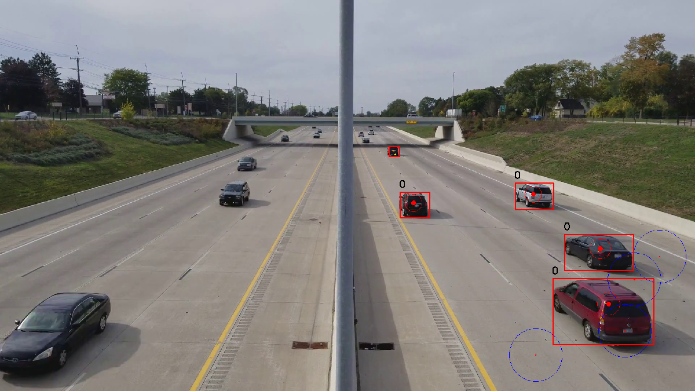
\includegraphics[width=\linewidth]{../../../experiments/E1/V1/noPd/36}
        \caption{Frame number: 36.}
        \label{fig:E1-V1-S0:01}
    \end{subfigure}
    \begin{subfigure}{0.48\textwidth}
        \centering
        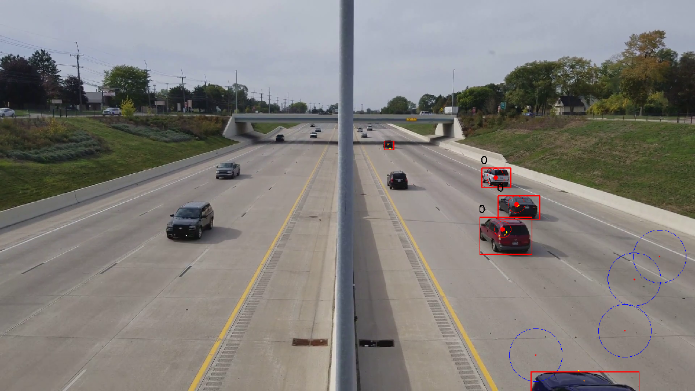
\includegraphics[width=\linewidth]{../../../experiments/E1/V1/noPd/48}
        \caption{Frame number: 48.}
        \label{fig:E1-V1-S0:02}
    \end{subfigure}
    \\
    \begin{subfigure}{0.48\textwidth}
        \centering
        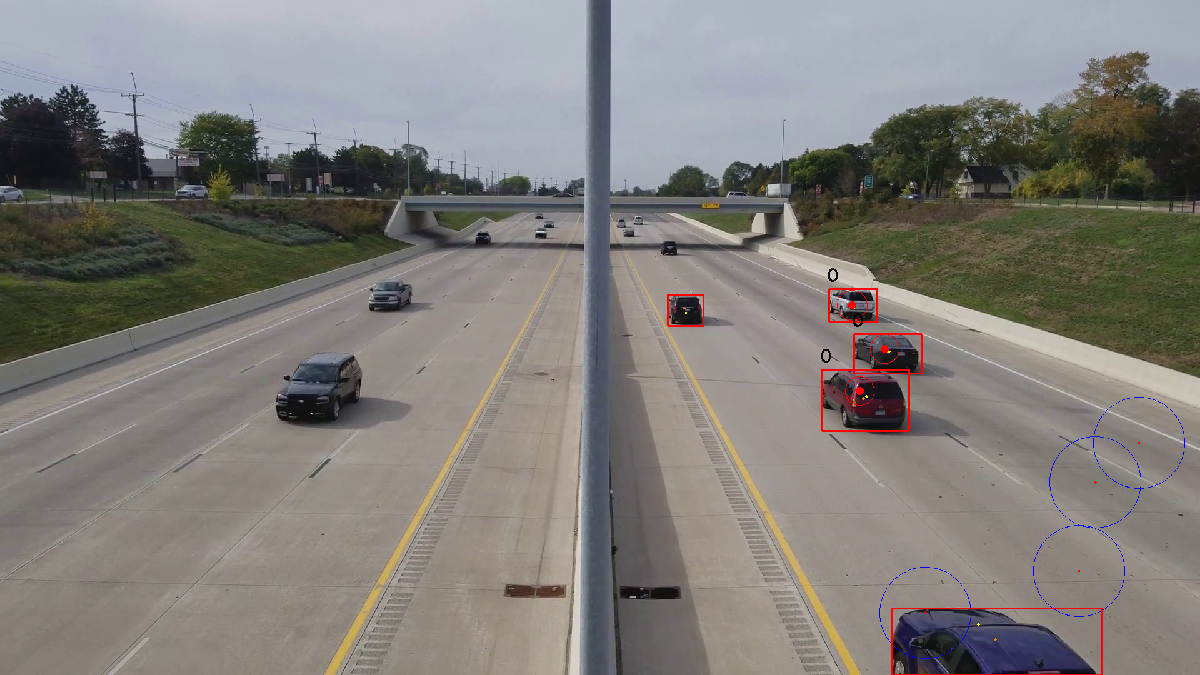
\includegraphics[width=\linewidth]{../../../experiments/E1/V1/noPd/49}
        \caption{Frame number: 49.}
        \label{fig:E1-V1-S0:03}
    \end{subfigure}
    \begin{subfigure}{0.48\textwidth}
        \centering
        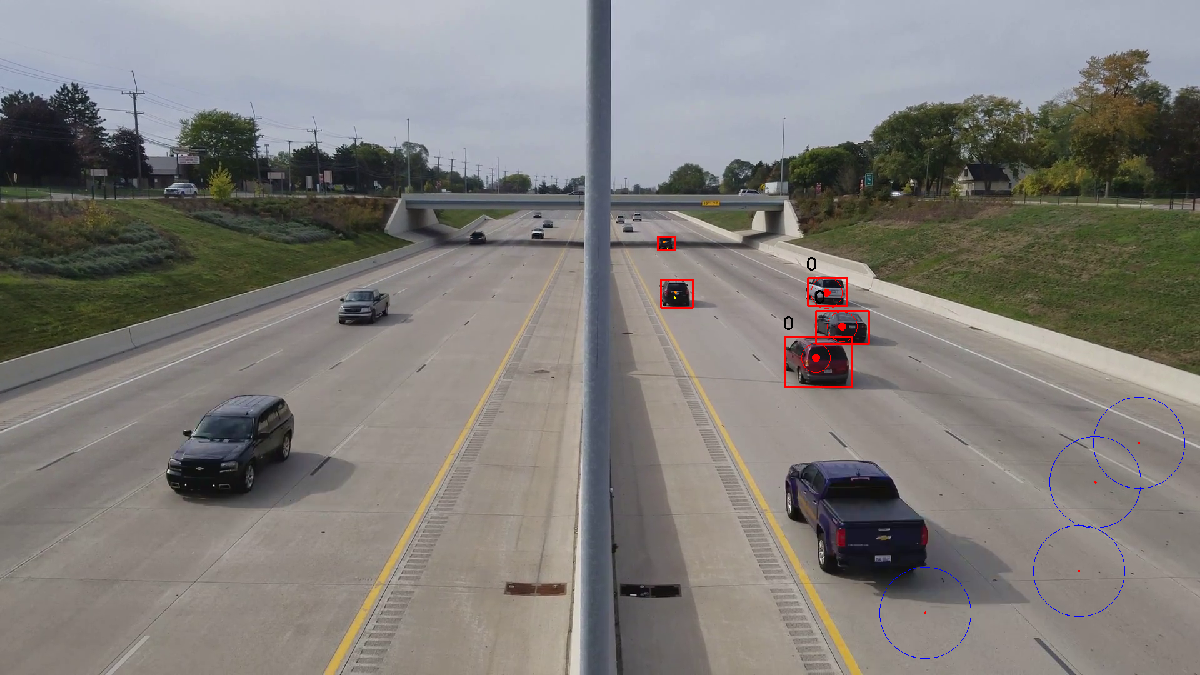
\includegraphics[width=\linewidth]{../../../experiments/E1/V1/noPd/56}
        \caption{Frame number: 56.}
        \label{fig:E1-V1-S0:04}
    \end{subfigure}
    \\
    \begin{subfigure}{0.48\textwidth}
        \centering
        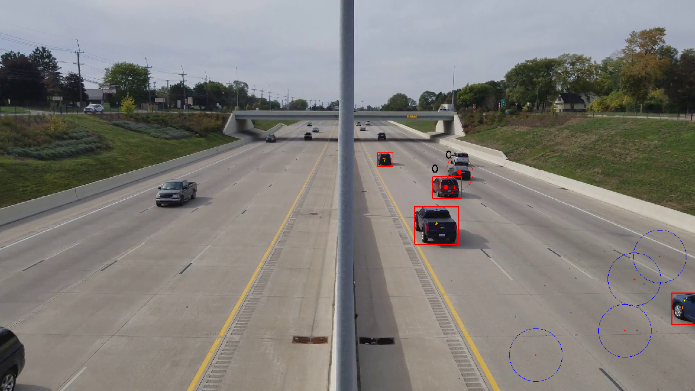
\includegraphics[width=\linewidth]{../../../experiments/E1/V1/noPd/67}
        \caption{Frame number: 67.}
        \label{fig:E1-V1-S0:05}
    \end{subfigure}
    \begin{subfigure}{0.48\textwidth}
        \centering
        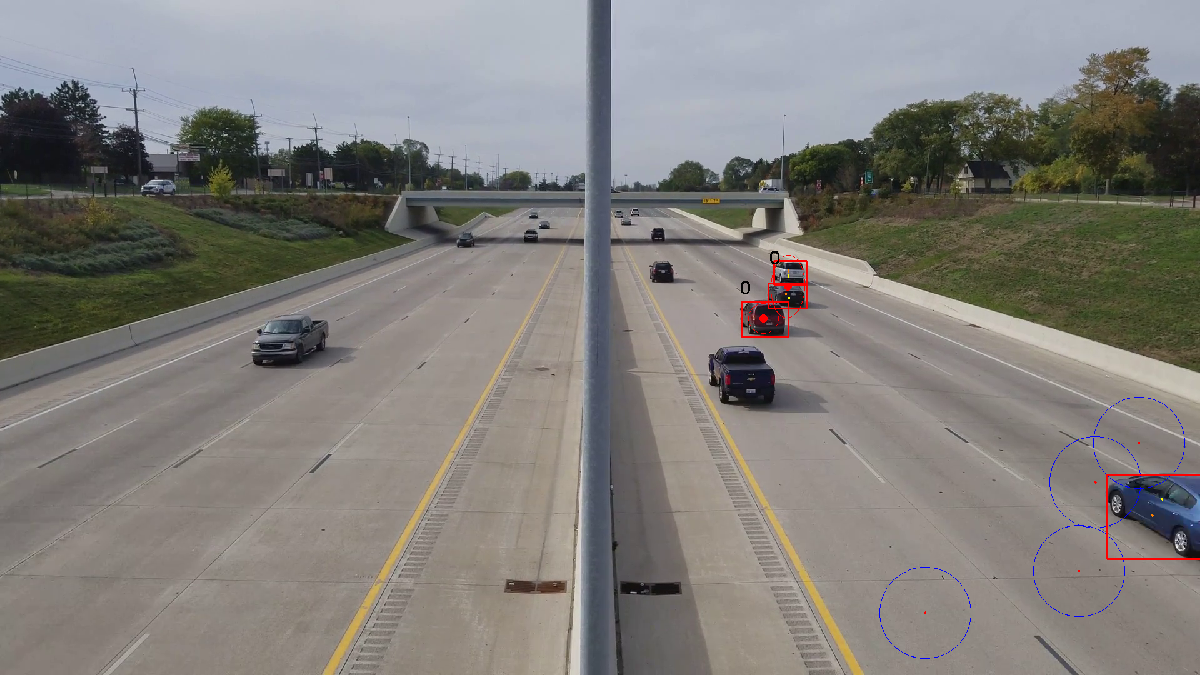
\includegraphics[width=\linewidth]{../../../experiments/E1/V1/noPd/69}
        \caption{Frame number: 69.}
        \label{fig:E1-V1-S0:06}
    \end{subfigure}
    \\
    \begin{subfigure}{0.48\textwidth}
        \centering
        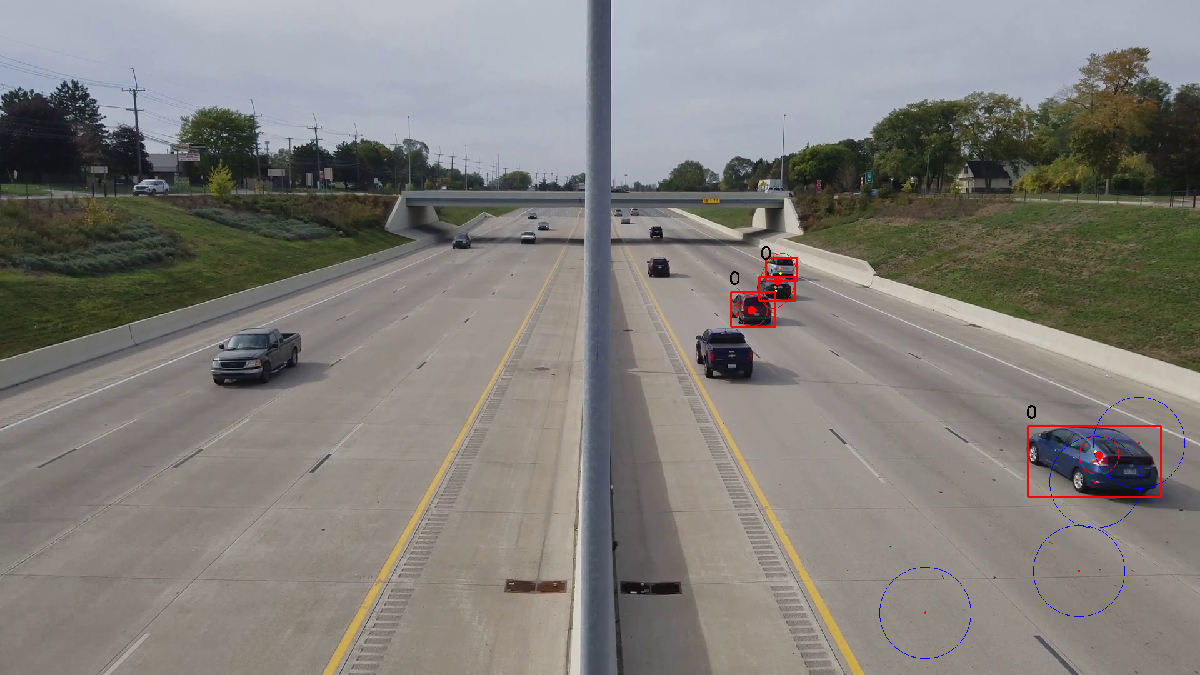
\includegraphics[width=\linewidth]{../../../experiments/E1/V1/noPd/73}
        \caption{Frame number: 73.}
        \label{fig:E1-V1-S0:07}
    \end{subfigure}
    \begin{subfigure}{0.48\textwidth}
        \centering
        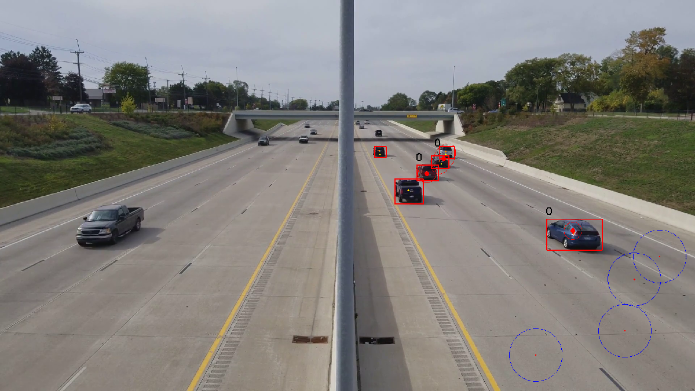
\includegraphics[width=\linewidth]{../../../experiments/E1/V1/noPd/79}
        \caption{Frame number: 79.}
        \label{fig:E1-V1-S0:08}
    \end{subfigure}
    \caption{Image sequence of tracked objects using the GM-PHD filter with constant detection probability.}
    \label{fig:E1-V1-S0}
\end{figure}

\subsection{V1 -- GM-PHD with the dynamic detection probability}
Following experiments test the GM-PHD filter with the dynamic detection probability and the modified pruning in the
video \textit{V1}.
\subsubsection{S1 -- YOLO + YOLO}
This experiment enhances settings \textit{S1}, i.e, the YOLO model provides both object detection bboxes and
segmentation masks.
The parameter settings are shown in Table \ref{tab:E1-V1-S1}.
\begin{table}[H]
    \centering
    \begin{tabular}{|c|c|c|c|c|c|c|c|c|}
        \hline
        $P_{D,k}(x)$ & $P$ & $\sigma_{\upsilon}$ & $\sigma_{\epsilon}$ & $T_H$ & $T_d$ & $T_p$ & $T_l$ & $T_{YOLO}$ \\ \noalign{\hrule
        height 1.5pt}
        0.3 & $diag(600,600,600,600)$ & 0.1 & 150 & 1 & 3 & 0.1 & 0.01 & 0.3\\
        \hline
    \end{tabular}
    \caption{The parameter settings for Experiment E1-V1-S1 with the dynamic detection probability.}
    \label{tab:E1-V1-S1}
\end{table}

Figure \ref{fig:E1-V1-S1} illustrates the performance of the GM-PHD filter under the dynamic detection probability and
settings \textit{S1}.

\begin{itemize}
    \item \textbf{\ref{fig:E1-V1-S1:01}:} Similarly as in the previous experiment, the initial frame presents four
    previously detected cars. Although a distant car is detected, it remains uninitialized since it has not crossed any spawning point.
    \item \textbf{\ref{fig:E1-V1-S1:02}:} By frame 48, the car on the left, which was undetected in the previous
    experiment, remains so. However, due to the elevated detection probability and adjusted pruning, the target manages to persist.
    \item \textbf{\ref{fig:E1-V1-S1:03}:} Despite the previous misdetections, the previously undetected car is once
    again
    identified, and the target successfully survives.
    \item \textbf{\ref{fig:E1-V1-S1:04}:} A new car crosses the spawning point, yet the YOLO model consistently fails to detect it over numerous consecutive frames, resulting in its non-initialization.
    \item \textbf{\ref{fig:E1-V1-S1:05}:} Two cars on the right evade the detection, yet their respective targets
    remain.
    \item \textbf{\ref{fig:E1-V1-S1:06}:} The previously undetected cars are once again identified, and both targets
    receive measurements, augmenting their weights.
    \item \textbf{\ref{fig:E1-V1-S1:07}:} Another car enters the scene and is successfully initialized.
    \item \textbf{\ref{fig:E1-V1-S1:08}:} The previously undetected car on the left merges with other targets.
    Consequently, this target is initialized despite the previous frequent misdetections. As a result, six true targets
    and six tracked targets are present.
\end{itemize}


The graph presented in \ref{gr:E1-V1-S1} showcases the enhanced performance of the GM-PHD filter. While all
targets do not immediately appear in the scene upon detection, they often still exist in the queue of targets
whose weights
have
not reached a threshold for display. However, upon receiving measurements, these targets' weights increase, leading to their reappearance in the scene.

This improvement is notable not only in the alignment of displayed targets with the true target count, but also in
the queue of potential targets exceeding the true count. Consequently, we gain awareness of potential targets that may manifest in the scene.


\begin{figure}[H]
    \centering
    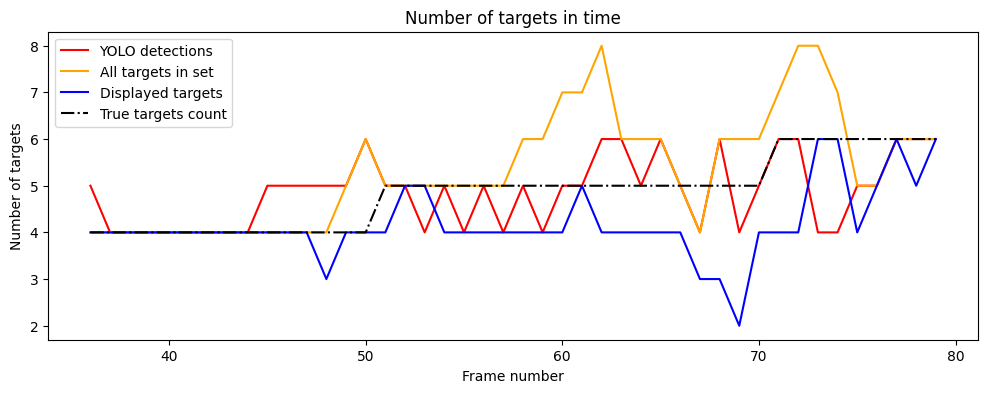
\includegraphics[width=\linewidth]{../../../experiments/E1/V1/YOLO/yolo_det}
    \caption{Development chart of the number of detected targets, targets in the filter's queue, displayed targets and
    the true
    targets' count.}
    \label{gr:E1-V1-S1}
\end{figure}

\begin{figure}[H]
    \centering
    \begin{subfigure}{0.48\textwidth}
        \centering
        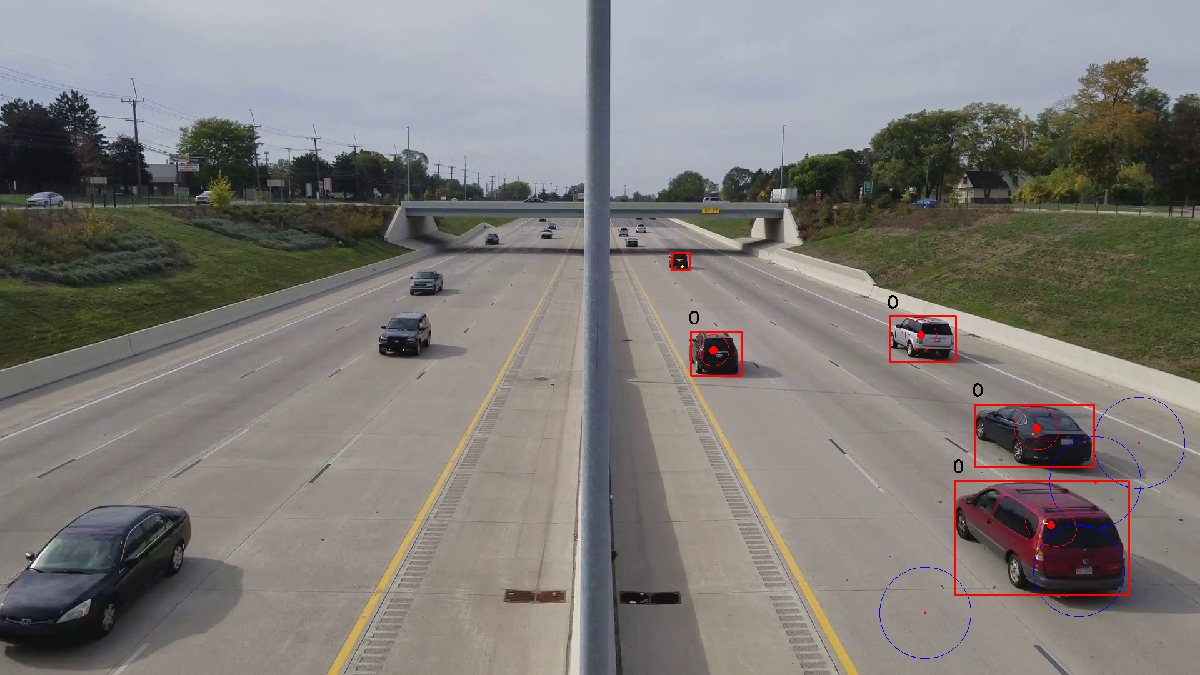
\includegraphics[width=\linewidth]{../../../experiments/E1/V1/YOLO/36}
        \caption{Frame number: 36.}
        \label{fig:E1-V1-S1:01}
    \end{subfigure}
    \begin{subfigure}{0.48\textwidth}
        \centering
        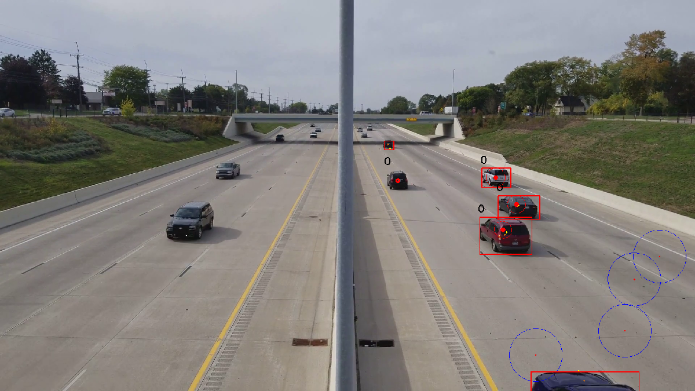
\includegraphics[width=\linewidth]{../../../experiments/E1/V1/YOLO/48}
        \caption{Frame number: 48.}
        \label{fig:E1-V1-S1:02}
    \end{subfigure}
    \\
    \begin{subfigure}{0.48\textwidth}
        \centering
        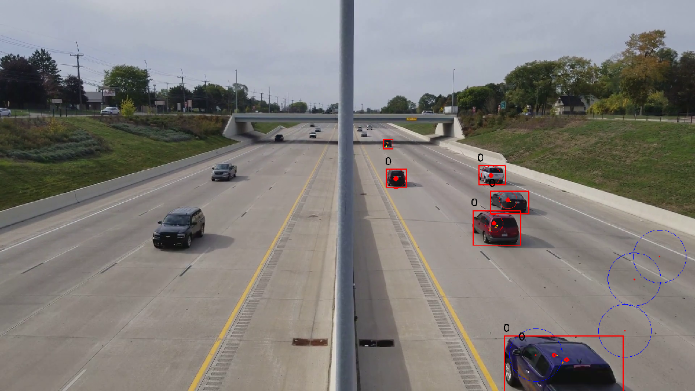
\includegraphics[width=\linewidth]{../../../experiments/E1/V1/YOLO/50}
        \caption{Frame number: 50.}
        \label{fig:E1-V1-S1:03}
    \end{subfigure}
    \begin{subfigure}{0.48\textwidth}
        \centering
        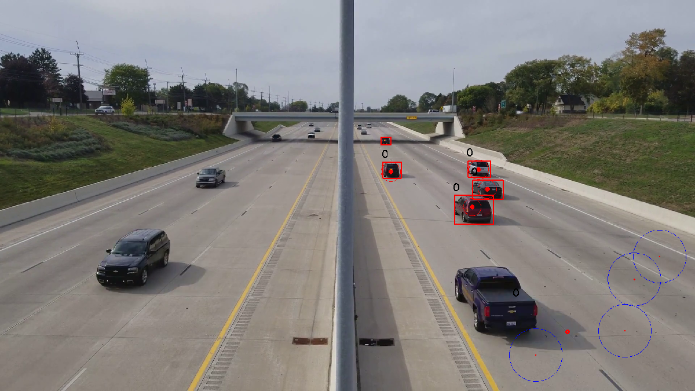
\includegraphics[width=\linewidth]{../../../experiments/E1/V1/YOLO/56}
        \caption{Frame number: 56.}
        \label{fig:E1-V1-S1:04}
    \end{subfigure}
    \\
    \begin{subfigure}{0.48\textwidth}
        \centering
        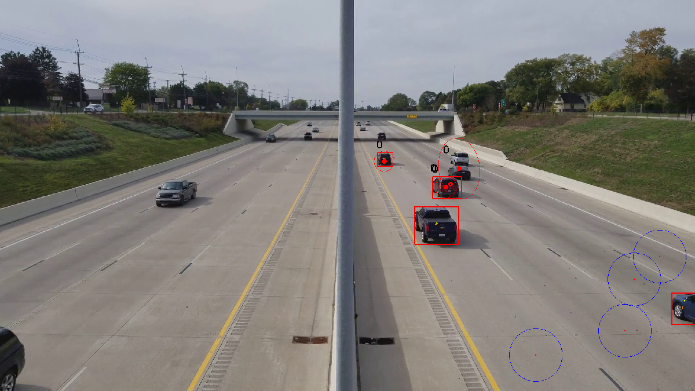
\includegraphics[width=\linewidth]{../../../experiments/E1/V1/YOLO/67}
        \caption{Frame number: 67.}
        \label{fig:E1-V1-S1:05}
    \end{subfigure}
    \begin{subfigure}{0.48\textwidth}
        \centering
        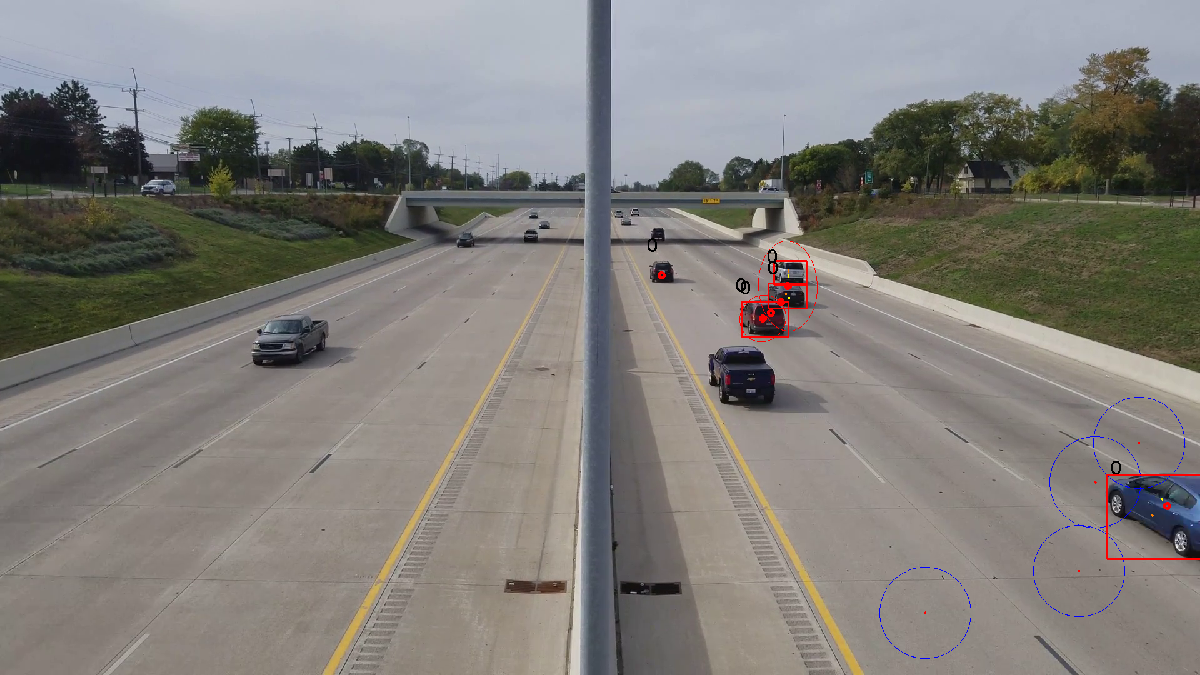
\includegraphics[width=\linewidth]{../../../experiments/E1/V1/YOLO/69}
        \caption{Frame number: 69.}
        \label{fig:E1-V1-S1:06}
    \end{subfigure}
    \\
    \begin{subfigure}{0.48\textwidth}
        \centering
        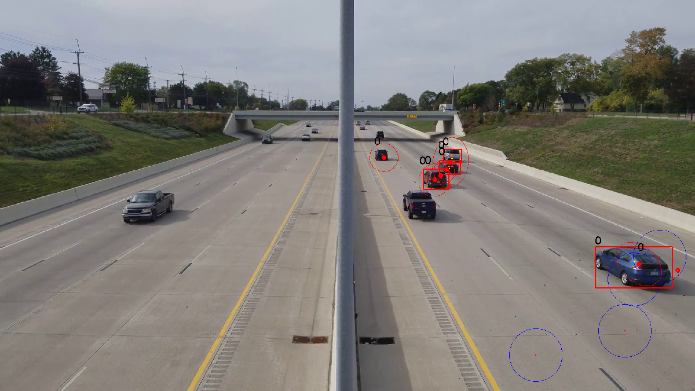
\includegraphics[width=\linewidth]{../../../experiments/E1/V1/YOLO/73}
        \caption{Frame number: 73.}
        \label{fig:E1-V1-S1:07}
    \end{subfigure}
    \begin{subfigure}{0.48\textwidth}
        \centering
        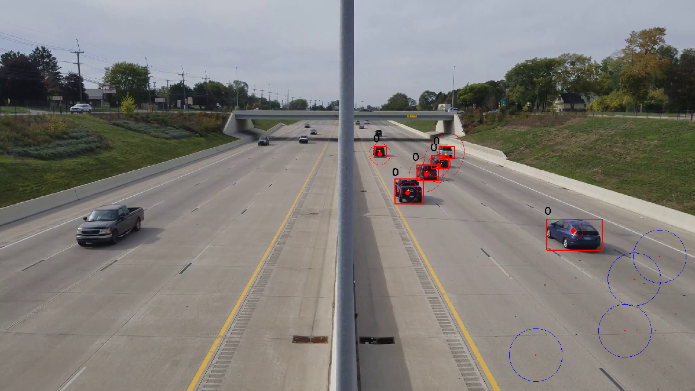
\includegraphics[width=\linewidth]{../../../experiments/E1/V1/YOLO/79}
        \caption{Frame number: 79.}
        \label{fig:E1-V1-S1:08}
    \end{subfigure}
    \caption{Image sequence of tracked objects using the GM-PHD filter with dynamic detection probability and YOLO
    only.}
    \label{fig:E1-V1-S1}
\end{figure}







\subsubsection{S2 -- YOLO + SAM}
This experiment employs configuration \textit{S2}, wherein the YOLO model furnishes objects' bounding boxes and the SAM model furnishes segmentation masks.
The parameter configurations can be found in Table \ref{tab:E1-V1-S2}.
\begin{table}[H]
    \centering
    \begin{tabular}{|c|c|c|c|c|c|c|c|c|}
        \hline
        $P_{D,k}(x)$ & $P$ & $\sigma_{\upsilon}$ & $\sigma_{\epsilon}$ & $T_H$ & $T_d$ & $T_p$ & $T_l$ & $T_{YOLO}$ \\ \noalign{\hrule
        height 1.5pt}
        0.3 & $diag(600,600,600,600)$ & 0.1 & 150 & 1 & 3 & 0.1 & 0.01 & 0.3\\
        \hline
    \end{tabular}
    \caption{The parameter settings for Experiment E1-V1-S2 with the dynamic detection probability.}
    \label{tab:E1-V1-S2}
\end{table}

Figure \ref{fig:E1-V1-S2} illustrates the GM-PHD filter's performance with the dynamic detection probability, employing
settings \textit{S2}.
This sequence is very similar to the previous experiment. There are four targets at the beginning and they are
tracked successfully the whole time. In the frame \ref{fig:E1-V1-S2:06} two of the targets are not detected, but both
survive. The YOLO model is not able to detect the fifth car, but it is initialized later due to the other target.

The graph \ref{gr:E1-V1-S2} shows a better stability in keeping the number of tracked targets. This might be caused by
the fact,
that the object detection YOLO model gives slightly different results than the object detection YOLO model with
segmentation capabilities. Furthermore, the "All targets in set" orange line, representing the number of targets in the
filter's queue, is more
accurate to the true count, deflecting only by one target at maximum.

Settings \textit{S2} perform manage a slightly better performance than settings \textit{S1}. The number of tracked
objects
is closer to
the true count.

\begin{figure}[H]
    \centering
    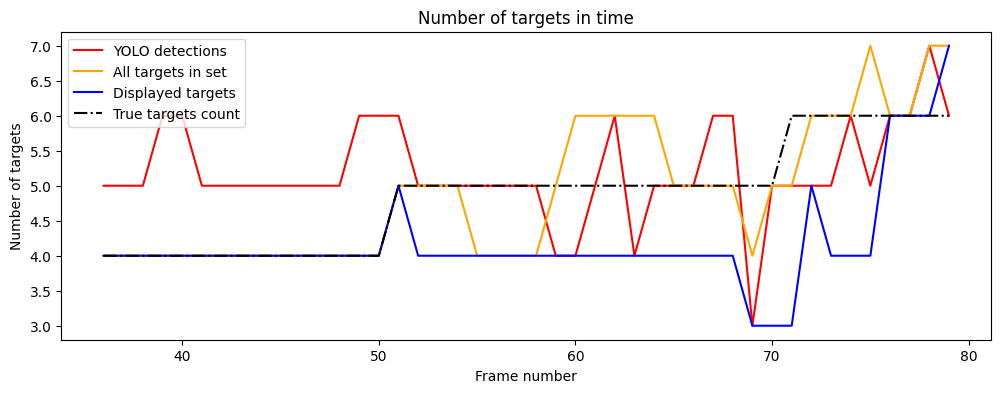
\includegraphics[width=\linewidth]{../../../experiments/E1/V1/SAM/sam_det}
    \caption{Development chart of the number of detected targets, targets in the filter's queue, displayed targets and
    the true
    targets' count.}
    \label{gr:E1-V1-S2}
\end{figure}

\begin{figure}[H]
    \centering
    \begin{subfigure}{0.48\textwidth}
        \centering
        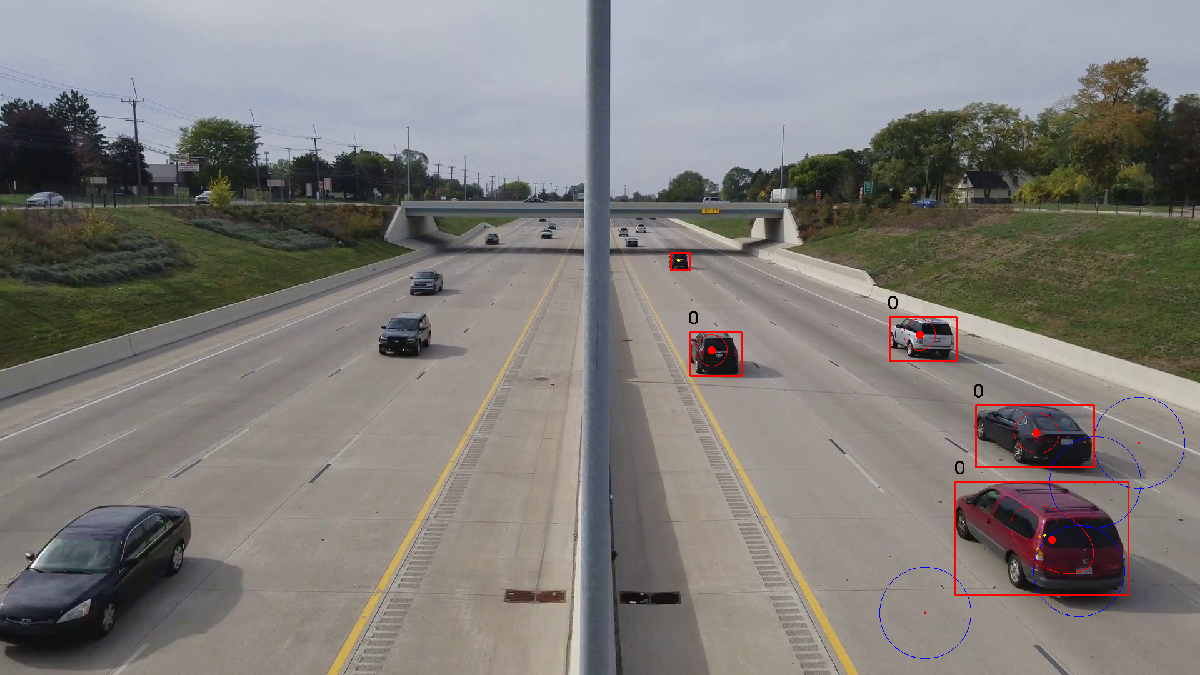
\includegraphics[width=\linewidth]{../../../experiments/E1/V1/SAM/36}
        \caption{Frame number: 36.}
        \label{fig:E1-V1-S2:01}
    \end{subfigure}
    \begin{subfigure}{0.48\textwidth}
        \centering
        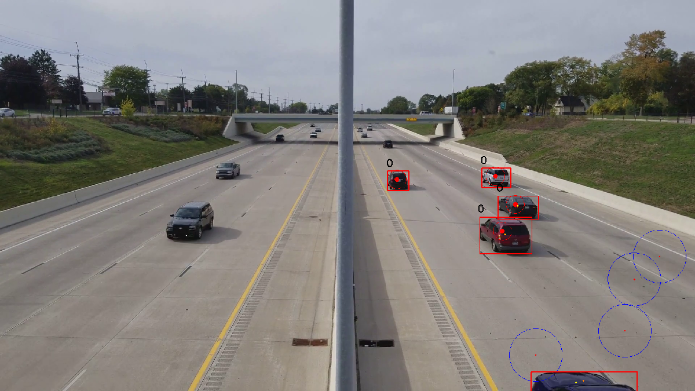
\includegraphics[width=\linewidth]{../../../experiments/E1/V1/SAM/48}
        \caption{Frame number: 48.}
        \label{fig:E1-V1-S2:02}
    \end{subfigure}
    \\
    \begin{subfigure}{0.48\textwidth}
        \centering
        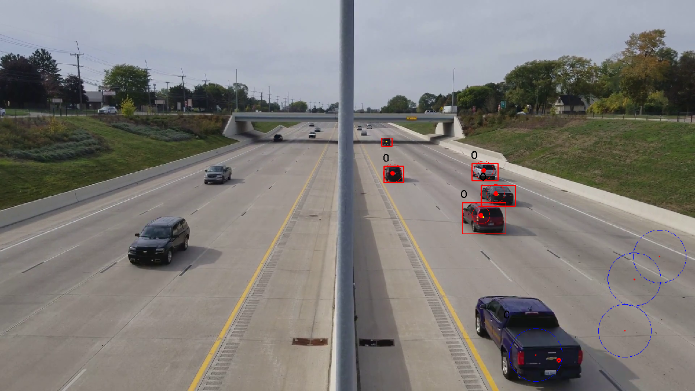
\includegraphics[width=\linewidth]{../../../experiments/E1/V1/SAM/53}
        \caption{Frame number: 53.}
        \label{fig:E1-V1-S2:03}
    \end{subfigure}
    \begin{subfigure}{0.48\textwidth}
        \centering
        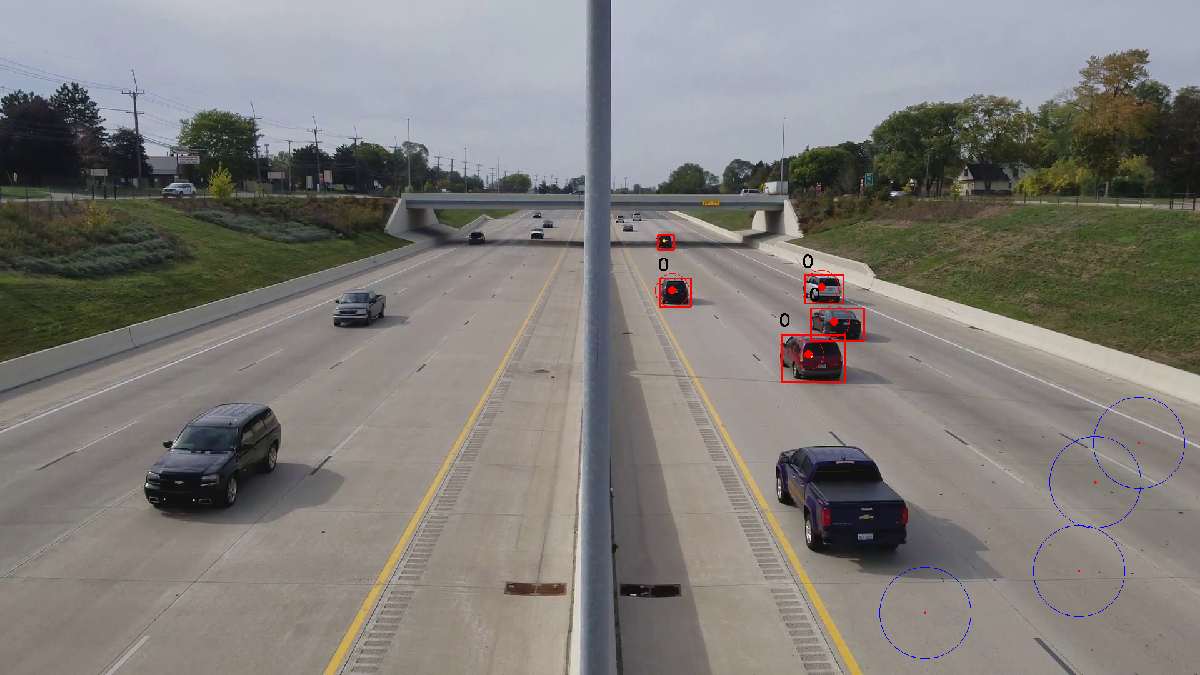
\includegraphics[width=\linewidth]{../../../experiments/E1/V1/SAM/57}
        \caption{Frame number: 57.}
        \label{fig:E1-V1-S2:04}
    \end{subfigure}
    \\
    \begin{subfigure}{0.48\textwidth}
        \centering
        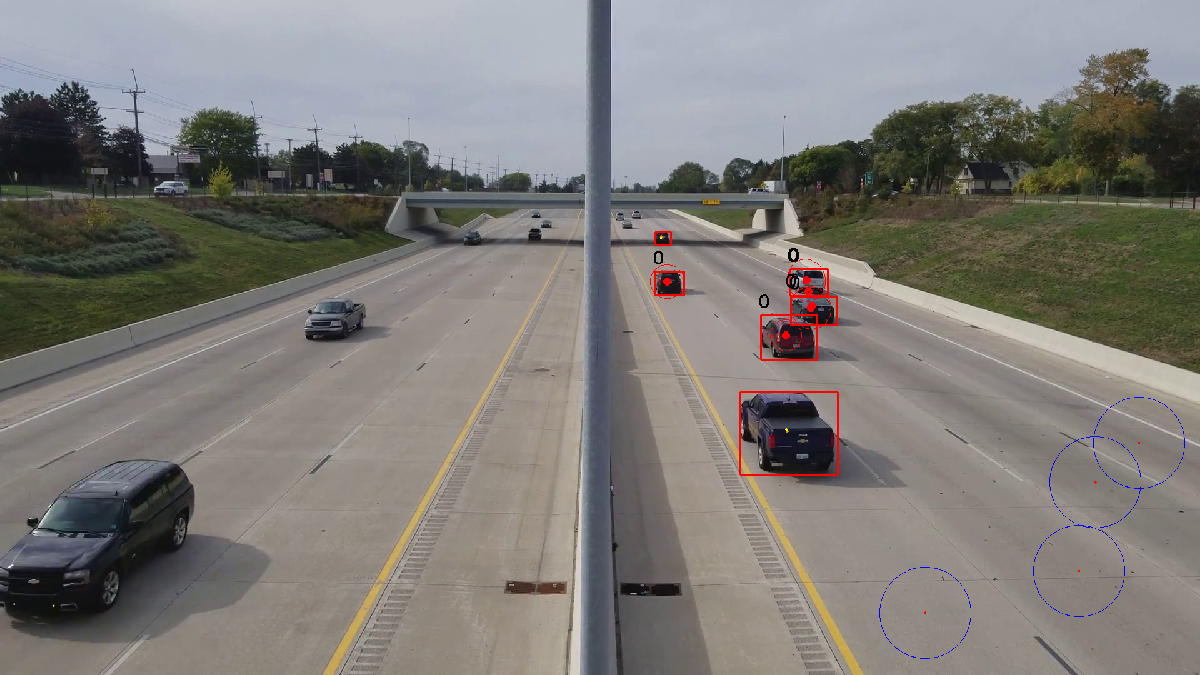
\includegraphics[width=\linewidth]{../../../experiments/E1/V1/SAM/62}
        \caption{Frame number: 62.}
        \label{fig:E1-V1-S2:05}
    \end{subfigure}
    \begin{subfigure}{0.48\textwidth}
        \centering
        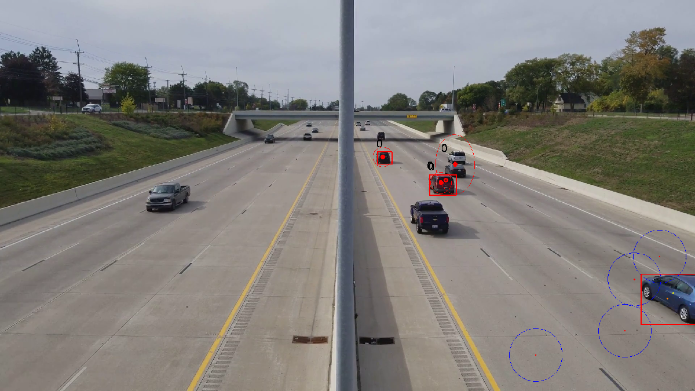
\includegraphics[width=\linewidth]{../../../experiments/E1/V1/SAM/69}
        \caption{Frame number: 69.}
        \label{fig:E1-V1-S2:06}
    \end{subfigure}
    \\
    \begin{subfigure}{0.48\textwidth}
        \centering
        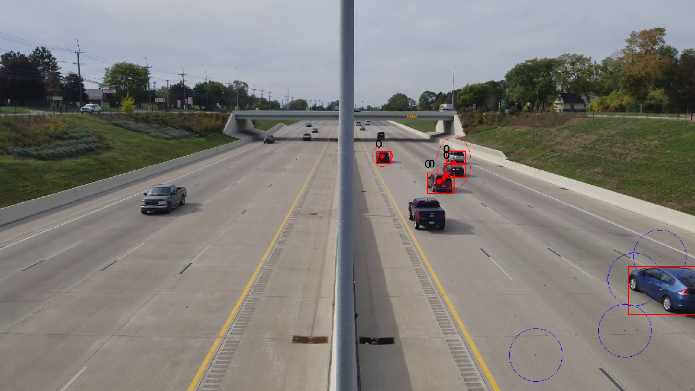
\includegraphics[width=\linewidth]{../../../experiments/E1/V1/SAM/70}
        \caption{Frame number: 70.}
        \label{fig:E1-V1-S2:07}
    \end{subfigure}
    \begin{subfigure}{0.48\textwidth}
        \centering
        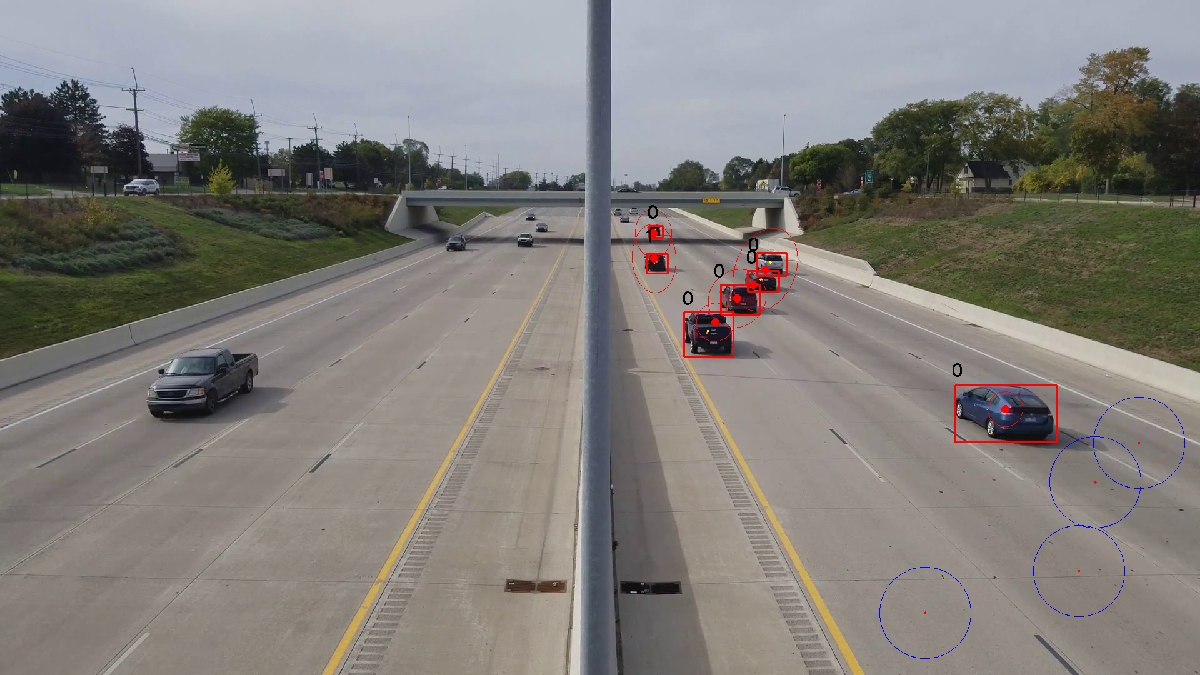
\includegraphics[width=\linewidth]{../../../experiments/E1/V1/SAM/78}
        \caption{Frame number: 78.}
        \label{fig:E1-V1-S2:08}
    \end{subfigure}
    \caption{Image sequence of tracked objects using the GM-PHD filter with the dynamic detection probability, the YOLO
    object detector and the SAM image segmentation model.}
    \label{fig:E1-V1-S2}
\end{figure}


\subsubsection{S3 -- Grounded SAM}
The experiment with settings \textit{S3} uses Grounding DINO object detector and the SAM image segmentation model.
All used parameters are included in Table \ref{tab:E1-V1-S3}.
\begin{table}[H]
    \centering
    \begin{tabular}{|c|c|c|c|c|c|c|c|c|c|}
        \hline
        $P_{D,k}(x)$ & $P$ & $\sigma_{\upsilon}$ & $\sigma_{\epsilon}$ & $T_H$ & $T_d$ & $T_p$ & $T_l$ & $T_{text}$ & $T_{bbox}$\\ \noalign{\hrule
        height 1.5pt}
        0.3 & $diag(600,600,600,600)$ & 0.1 & 150 & 1 & 3 & 0.1 & 0.01 & 0.3 & 0.3\\
        \hline
    \end{tabular}
    \caption{The parameter settings for Experiment E1-V1-S3 with the dynamic detection probability.}
    \label{tab:E1-V1-S3}
\end{table}

Figure \ref{fig:E1-V1-S3} shows the performance of the GM-PHD filter with the dynamic detection probability with settings \textit{S3}.
\begin{itemize}
    \item \textbf{\ref{fig:E1-V1-S3:01}:} The utilization of a distinct object detection model results in an
    increased number of cars detected within the scene. However, only the four cars in the front have driven through
    the spawn
    points thus are considered within the true count.
    \item \textbf{\ref{fig:E1-V1-S3:02}:} All targets are effectively tracked without any issues.
    \item \textbf{\ref{fig:E1-V1-S3:03}:} Unlike YOLO, Grounding DINO successfully detects the arrival of a new car.
    \item In \textbf{\ref{fig:E1-V1-S3:04}, \ref{fig:E1-V1-S3:05}, \ref{fig:E1-V1-S3:06}} no events of greater
    importance occur.
    \item \textbf{\ref{fig:E1-V1-S3:07}:} Subsequently, the following arriving car is promptly detected and initialized.
    \item \textbf{\ref{fig:E1-V1-S3:08}:} This frame presents new challenges. Given the decreased distance between
    the cars and their proximity to each other, coupled with the model's ability to detect all of the cars, an excess of
    new
    targets emerges. To address this issue, adjustments to the motion noise are necessary. Additionally, for
    such scenarios, the implementation of the dynamic motion noise and the observation noise could offer a viable
    solution.
\end{itemize}

Graph \ref{gr:E1-V1-S3} shows, that the number of detected objects is far beyond the true count. Nevertheless,
the number of displayed targets is almost on spot till the frame 66. As the targets get closer to each
other, the
number of targets grows rapidly, causing errors to the number of tracked objects.

This setting outperforms the other settings. The performance of Grounding DINO brings another problems arising from
characteristics of the video. The video is taken from an angle, which makes the cars smaller as they carry on. These
dynamics align poorly with the static motion and the observation noise.

\begin{figure}[H]
    \centering
    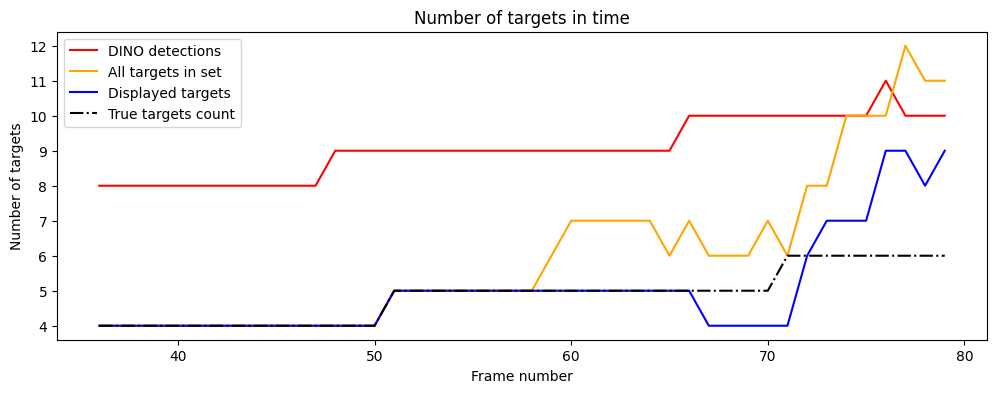
\includegraphics[width=\linewidth]{../../../experiments/E1/V1/DINO/dino_det}
    \caption{Development chart of the number of detected targets, targets in the filter's queue, displayed targets
    and the
    true
    targets' count.}
    \label{gr:E1-V1-S3}
\end{figure}

\begin{figure}[H]
    \centering
    \begin{subfigure}{0.48\textwidth}
        \centering
        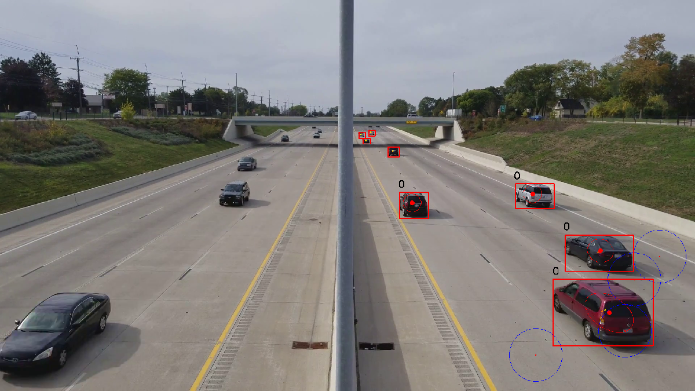
\includegraphics[width=\linewidth]{../../../experiments/E1/V1/DINO/36}
        \caption{Frame number: 36.}
        \label{fig:E1-V1-S3:01}
    \end{subfigure}
    \begin{subfigure}{0.48\textwidth}
        \centering
        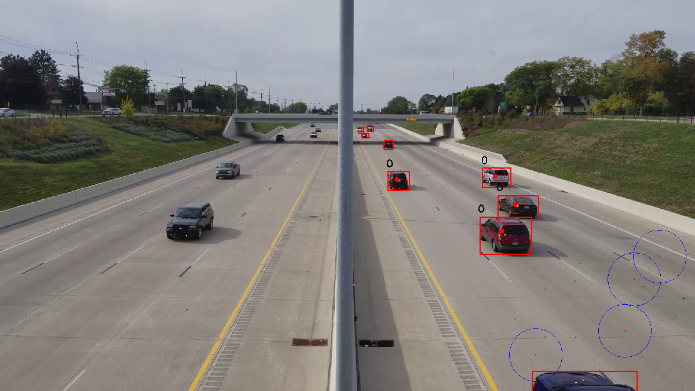
\includegraphics[width=\linewidth]{../../../experiments/E1/V1/DINO/48}
        \caption{Frame number: 48.}
        \label{fig:E1-V1-S3:02}
    \end{subfigure}
    \\
    \begin{subfigure}{0.48\textwidth}
        \centering
        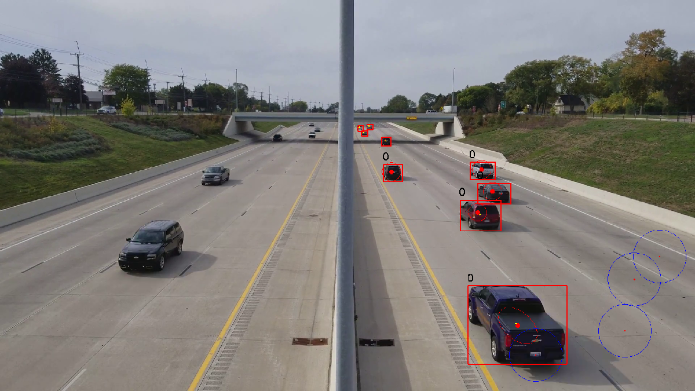
\includegraphics[width=\linewidth]{../../../experiments/E1/V1/DINO/54}
        \caption{Frame number: 54.}
        \label{fig:E1-V1-S3:03}
    \end{subfigure}
    \begin{subfigure}{0.48\textwidth}
        \centering
        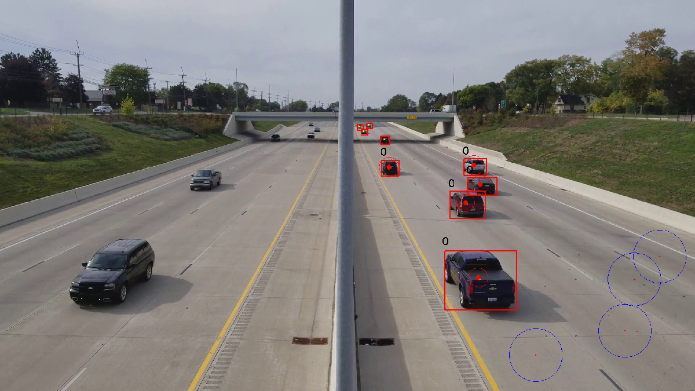
\includegraphics[width=\linewidth]{../../../experiments/E1/V1/DINO/58}
        \caption{Frame number: 58.}
        \label{fig:E1-V1-S3:04}
    \end{subfigure}
    \\
    \begin{subfigure}{0.48\textwidth}
        \centering
        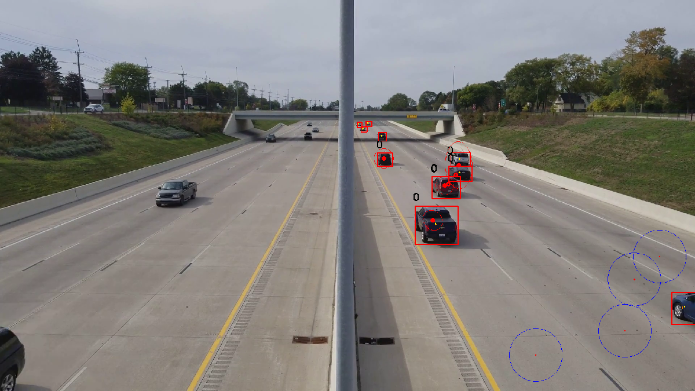
\includegraphics[width=\linewidth]{../../../experiments/E1/V1/DINO/67}
        \caption{Frame number: 67.}
        \label{fig:E1-V1-S3:05}
    \end{subfigure}
    \begin{subfigure}{0.48\textwidth}
        \centering
        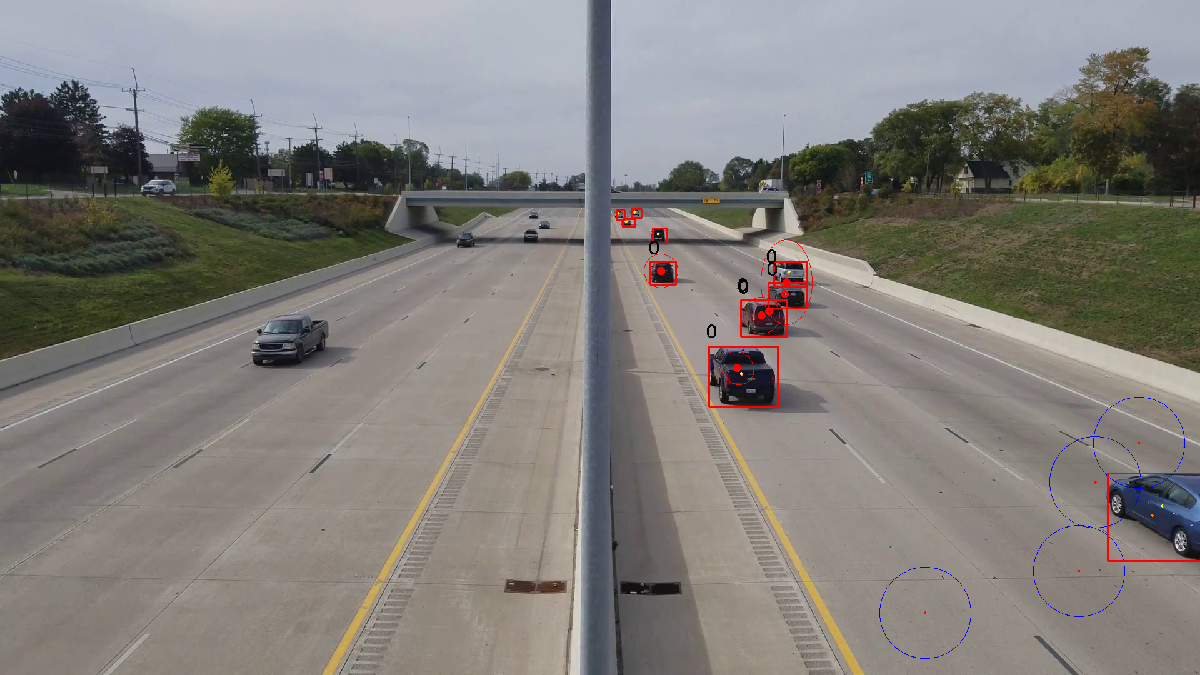
\includegraphics[width=\linewidth]{../../../experiments/E1/V1/DINO/69}
        \caption{Frame number: 69.}
        \label{fig:E1-V1-S3:06}
    \end{subfigure}
    \\
    \begin{subfigure}{0.48\textwidth}
        \centering
        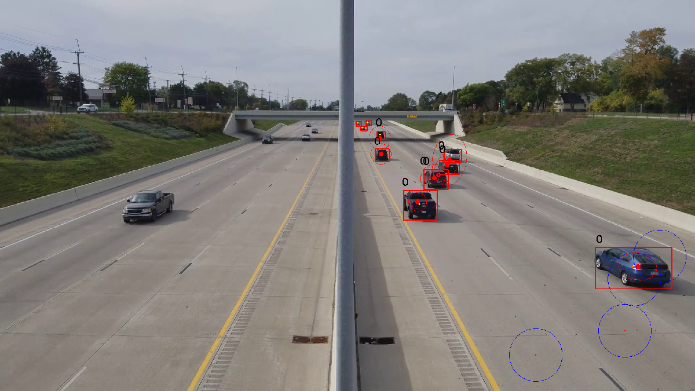
\includegraphics[width=\linewidth]{../../../experiments/E1/V1/DINO/73}
        \caption{Frame number: 73.}
        \label{fig:E1-V1-S3:07}
    \end{subfigure}
    \begin{subfigure}{0.48\textwidth}
        \centering
        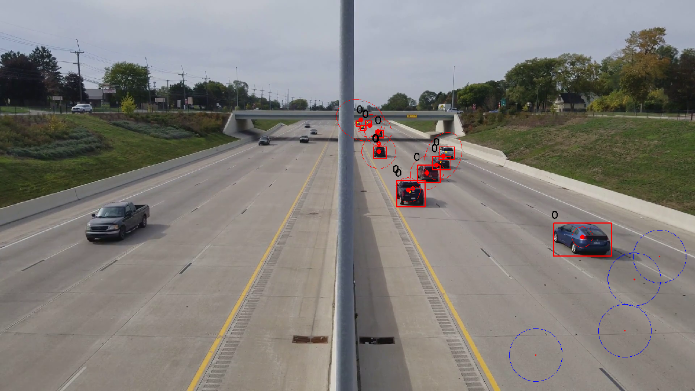
\includegraphics[width=\linewidth]{../../../experiments/E1/V1/DINO/78}
        \caption{Frame number: 79.}
        \label{fig:E1-V1-S3:08}
    \end{subfigure}
    \caption{Image sequence of tracked objects using the GM-PHD filter with the dynamic detection probability and
    the
    Grounded SAM model.}
    \label{fig:E1-V1-S3}
\end{figure}
